\documentclass[a4paper,12pt]{article}
\usepackage[a4paper, margin=2.5cm]{geometry}
\usepackage[pdftex]{graphicx}
\usepackage{tikz}
\usepackage{pgfplots}
\usepackage{enumitem}
\usepackage{float}
\usepackage[document]{ragged2e}
\usepackage[utf8]{inputenc}
\usepackage[T1]{fontenc}
\usepackage[spanish,es-tabla]{babel}
\renewcommand{\shorthandsspanish}{}
\usepackage{xurl}
\usepackage{lipsum}
\usepackage{mwe}
\usepackage{multicol}
\usepackage{siunitx}
\usepackage{listings}
\usepackage{enumitem}
\usepackage{amsmath}
\usepackage{listings}
\usepackage{tabularray}
\usepackage{xparse}
\usepackage{dsfont}
\usepackage{matlab-prettifier}

\graphicspath{ {/home/saikkopat/Documents/ESCOM/CAL/T03/MATLAB/} }

\NewDocumentCommand{\INTERVALINNARDS}{ m m }{
    #1 {,} #2
}
\NewDocumentCommand{\interval}{ s m >{\SplitArgument{1}{,}}m m o }{
    \IfBooleanTF{#1}{
        \left#2 \INTERVALINNARDS #3 \right#4
    }{
        \IfValueTF{#5}{
            #5{#2} \INTERVALINNARDS #3 #5{#4}
        }{
            #2 \INTERVALINNARDS #3 #4
        }
    }
}


\begin{document}

\begin{titlepage}
	\begin{tikzpicture}[overlay, remember picture]
		\path (current page.north east) ++(-0.3,-1.6) node[below left] {
\includegraphics[width=0.35\textwidth]{/home/saikkopat/Documents/LOGOS IPN/EscudoESCOM}};
	\end{tikzpicture}
	\begin{tikzpicture}[overlay, remember picture]
		\path (current page.north west) ++(1.5,-1) node[below right] {
\includegraphics[width=0.2\textwidth]{/home/saikkopat/Documents/LOGOS IPN/logo}};
	\end{tikzpicture}
	\begin{center}
		\vspace{-1.5cm}
		{\LARGE Instituto Politécnico Nacional\par}
		\vspace{.5cm}
		{\LARGE Escuela Superior de Cómputo\par}
		\vspace{2.5cm}
		{\large Unidad de aprendizaje:}\\{\Large Cálculo\par}
		\vspace{5cm}
		{\scshape\Huge Tarea 3:\par}
		{\itshape\Large Clasificación de funciones\par}
		\vfill
		{\Large Alumno:\par}
		\vspace{0.7cm}
		{\Large González Cárdenas Ángel Aquilez\par}
		\vspace{0.5cm}
		{\Large Boleta: 2016630152\par}
		\vspace{0.5cm}
		{\Large Grupo: 1CV8\par}
		\vspace{1cm}
		{\Large Profesor: Jurado Jiménez Roberto\par}
		\vfill
	\end{center}
\end{titlepage} 

\newpage

\section*{Clasificación de funciones}

Una función (también llamada \emph{aplicación}) entre dos \emph{conjuntos} se escribe de la forma:

\[	f: X \rightarrow Y\] \\

donde $X$ es el \emph{dominio}, $Y$ el \emph{rango}, \emph{contradominio} o \emph{imagen}.\par

También se escribe que $x \mapsto f(x)$.\par


\subsection*{Función inyectiva}

Una función es \emph{inyectiva} si para todo $a$, $b$ distintos, y que pertenecen a $X$, sus imágenes $f(a)$ y $f(b)$ son distintas. \\

Es decir, una función es inyectiva cuando las \textit{imágenes de elementos distintos son distintas}. \par

\[f : X \rightarrow Y \text{ es inyectiva } \iff \forall a, b \in X, a \neq b \implies f(a) \neq f(b) \]

Ejemplos:

\begin{enumerate}
	\centering
	\item Función identidad
		\begin{multicols}{2}
		Código \texttt{MATLAB}
		\begin{lstlisting}[style=Matlab-editor]
x = linspace(-10,10);
y = x;
plot(x,y)
title('f(x) = x')
xlabel('x')
ylabel('f(x)')
grid on
		\end{lstlisting}
		\columnbreak
			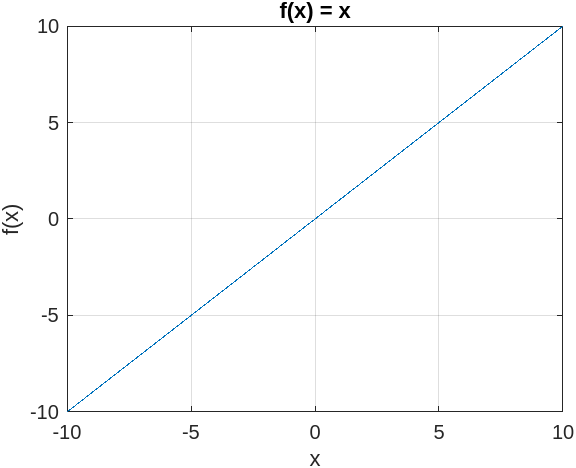
\includegraphics[width=0.5\textwidth]{FIG1}
		\end{multicols}
	
	\item Función exponencial
		\begin{multicols}{2}
		Código \texttt{MATLAB}
		\begin{lstlisting}[style=Matlab-editor]
x = linspace(-10,10);
y = exp(x);
plot(x,y)
title('f(x) = e^x')
xlabel('x')
ylabel('f(x)')
grid on
		\end{lstlisting}
		\columnbreak
			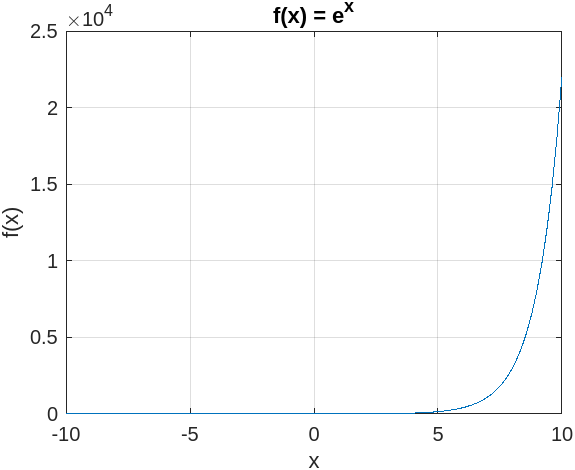
\includegraphics[width=0.5\textwidth]{FIG2}
		\end{multicols}

		\item Función logarítmica
		\begin{multicols}{2}
		Código \texttt{MATLAB}
		\begin{lstlisting}[style=Matlab-editor]
x = linspace(0.1,10);
y = log(x);
plot(x,y)
title('f(x) = ln(x)')
xlabel('x')
ylabel('f(x)')
grid on
		\end{lstlisting}
		\columnbreak
			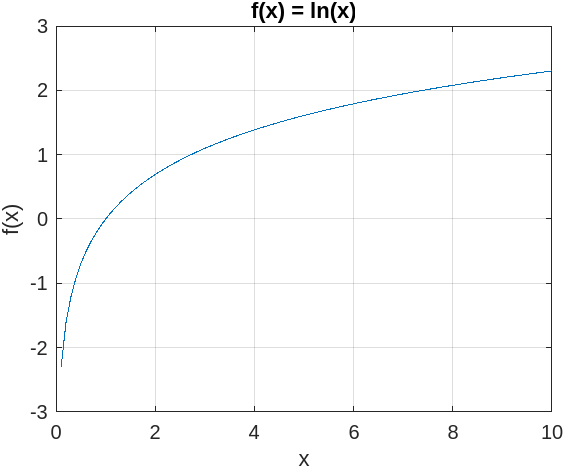
\includegraphics[width=0.5\textwidth]{FIG3}
		\end{multicols}

\end{enumerate}

\vspace{1cm}

\subsection*{Función sobreyectiva}

\vspace{1cm}

Una función es \emph{sobreyctiva} (o \emph{suprayectiva}) si todos los elementos de la imagen $Y$ tienen anti-imagen. Es decir, si para cualquier $y$ de la imagen $Y$ existe al menos un elemento $x$ de la imagen tal que $f(x) = y$. \\

Esta propiedad es independiente de la \emph{inyectividad}.

\[ \text{Si } f : X \rightarrow Y \text{ entonces se dice que } f \text{ es sobreyectiva si } \forall y \in Y, \exists x \in X : f(x) = y \] \\

\vspace{1cm}
Ejemplos:


\begin{enumerate}
	\centering
	\item Función lineal
		\begin{multicols}{2}
		Código \texttt{MATLAB}
		\begin{lstlisting}[style=Matlab-editor]
x = linspace(-10,10);
y = 2*x + 1;
plot(x,y)
title('f(x) = 2x + 1')
xlabel('x')
ylabel('f(x)')
grid on
		\end{lstlisting}
		\columnbreak
			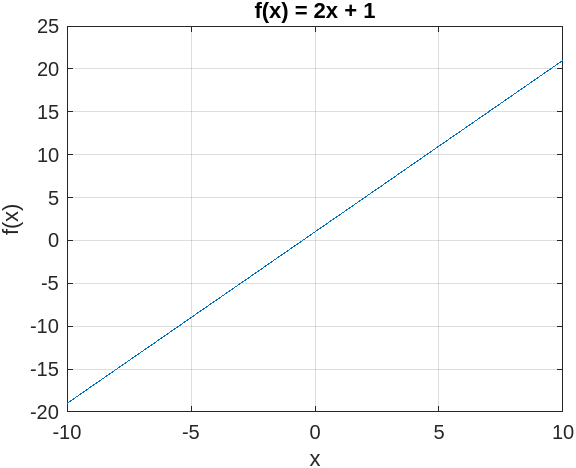
\includegraphics[width=0.5\textwidth]{FIG4}
		\end{multicols}
	
	\item Función cúbica
		\begin{multicols}{2}
		Código \texttt{MATLAB}
		\begin{lstlisting}[style=Matlab-editor]
x = linspace(-10,10);
y = x.^3;
plot(x,y)
title('f(x) = x^3')
xlabel('x')
ylabel('f(x)')
grid on
		\end{lstlisting}
		\columnbreak
			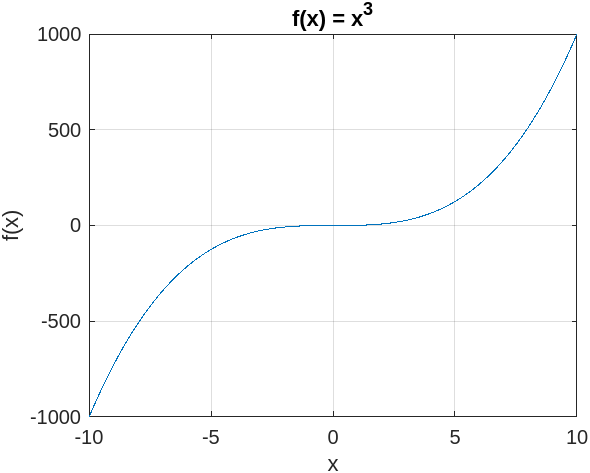
\includegraphics[width=0.5\textwidth]{FIG5}
		\end{multicols}

		\item Función senoidal
		\begin{multicols}{2}
		Código \texttt{MATLAB}
		\begin{lstlisting}[style=Matlab-editor]
x = linspace(-2*pi,2*pi);
y = sin(x);
plot(x,y)
title('f(x) = sin(x)')
xlabel('x')
ylabel('f(x)')
grid on
		\end{lstlisting}
		\columnbreak
			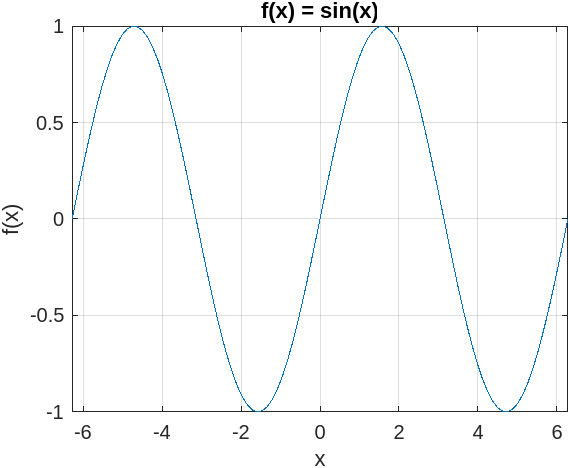
\includegraphics[width=0.5\textwidth]{FIG6}
		\end{multicols}

\end{enumerate}


\subsection*{Función biyectiva}

\vspace{1cm}

Una función es \emph{biyectiva} si es inyectiva y sobreyectiva. \\

En tal caso, existe una función $g$, llamada \emph{función inversa}, tal que para todo $x$ del dominio, 

\[g(f(x)) = x\] \\

y para todo $y$ de la imagen

\[ f(g(y)) = y \] \\

Normalmente, la función inversa de $f$ se denota por $f^{-1}$ en lugar de $g$. \\

\newpage

Ejemplos:

\begin{enumerate}
	\centering
	\item Función cuadrática: La función $f(x) = x^2$ es biyectiva en el intervalo $[0, \infty)$ y su inversa es 
	$f^-1(x) = sqrt(x)$.

	\vspace{1.5cm}
		\begin{multicols}{2}
		Código \texttt{MATLAB}
		\begin{lstlisting}[style=Matlab-editor]
x = linspace(0,5);
y = x.^2;
plot(x,y)
title('f(x) = x^2, f^-1 = sqrt(x)')
xlabel('x')
ylabel('f(x), f^-1(x)')
hold on
y_inv = sqrt(x);
plot(x,y_inv)
legend('f(x)','f^-1(x)')
grid on
hold off
		\end{lstlisting}
		\columnbreak
			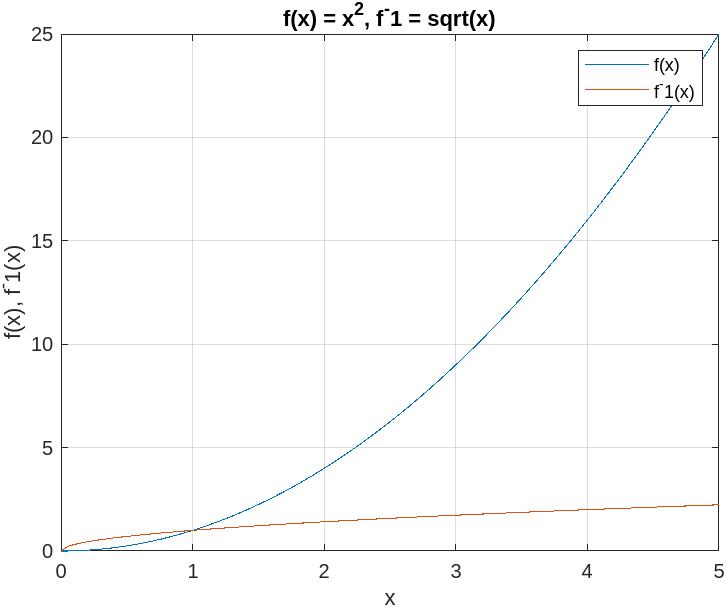
\includegraphics[width=0.5\textwidth]{FIG7}
		\end{multicols}
	
	\item  Función tangente: La función $f(x) = tan(x)$ es biyectiva en el intervalo $(-\dfrac{\pi}{2}, \dfrac{\pi}{2})$ y su inversa es $f^{-1}(x) = atan(x)$.
	 \vspace{1.5cm}
		\begin{multicols}{2}
		Código \texttt{MATLAB}
		\begin{lstlisting}[style=Matlab-editor]
x = linspace(-pi/2,pi/2);
y = tan(x);
plot(x,y)
title('f(x) = tan(x), f^-1(x) = atan(x)')
xlabel('x')
ylabel('f(x), f^-1(x)')
hold on
y_inv = atan(x);
plot(x,y_inv)
legend('f(x)','f^-1(x)')
grid on
hold off
		\end{lstlisting}
		\columnbreak
			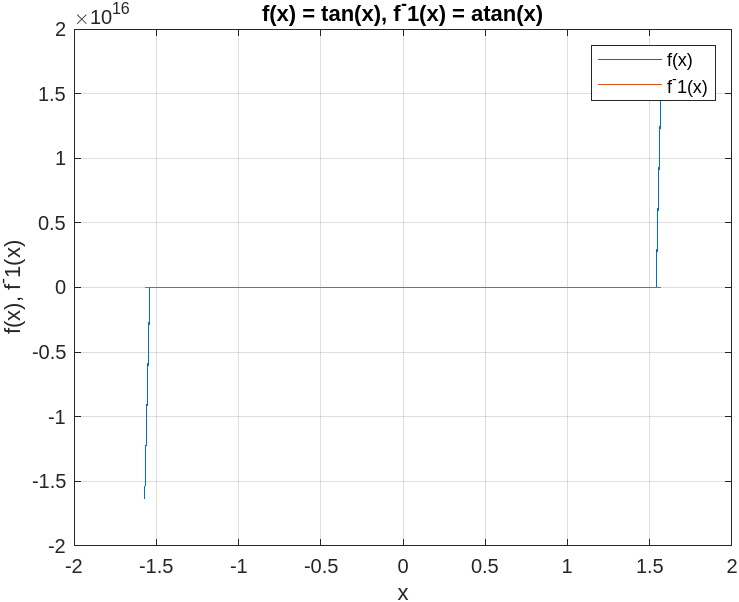
\includegraphics[width=0.5\textwidth]{FIG8}
		\end{multicols}

		\item Función raíz cuadrada: La función $f(x) = sqrt(x)$ es biyectiva en el intervalo $[0, \infty)$ y su inversa es $f^-1(x) = x^2$.
		 \vspace{1cm}
		\begin{multicols}{2}
		Código \texttt{MATLAB}
		\begin{lstlisting}[style=Matlab-editor]
x = linspace(0,5);
y = sqrt(x);
plot(x,y)
title('f(x) = sqrt(x), f^-1(x) = x^2')
xlabel('x')
ylabel('f(x), f^-1(x)')
hold on
y_inv = x.^2;
plot(x,y_inv)
legend('f(x)','f^-1(x)')
grid on
hold off
		\end{lstlisting}
		\columnbreak
			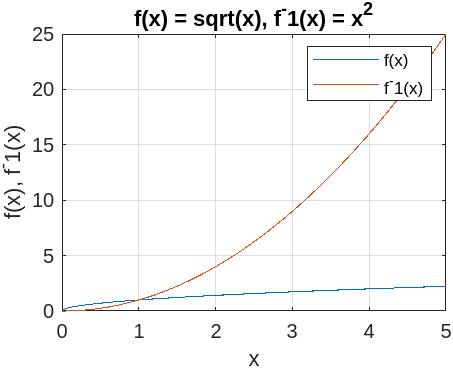
\includegraphics[width=0.5\textwidth]{FIG9}
		\end{multicols}

\end{enumerate}

Para calcular la inversa de una función en términos matemáticos, se procede de la siguiente forma:\\

1. Denotar la función $f(x)$ como $y = f(x)$.

2. Intercambiar $x$ y $y$ en la ecuación. Esto te dará una ecuación de la forma $x = f(y)$.

3. Resolver para $y$. La solución a esta ecuación será la función inversa, denotada como $$f^{-1}(x)$$.

Por ejemplo, si se tiene la función $$f(x) = 2x + 3$$, para encontrar la función inversa se procede:

1. Se denota la función como $$y = 2x + 3$$.
2. Se intercambia $x$ y $y$ para obtener $$x = 2y + 3$$.
3. Se resuelve para $$y$$ para obtener $$f^{-1}(x) = \frac{x - 3}{2}$$.

Por lo tanto, la inversa de la función $$f(x) = 2x + 3$$ es $$f^{-1}(x) = \frac{x - 3}{2}$$.


\end{document}